%% LyX 2.1.4 created this file.  For more info, see http://www.lyx.org/.
%% Do not edit unless you really know what you are doing.
\documentclass[12pt,english,ms]{report}
\usepackage{savesym}
\savesymbol{setlocale}
\usepackage{babel}
\restoresymbol{TXF}{setlocale}
\usepackage[T1]{fontenc}
\usepackage[latin9]{inputenc}
\usepackage{longtable}
\usepackage{float}
\usepackage{calc}
\usepackage{amsmath}
\usepackage{amsthm}
\usepackage{setspace}
\usepackage[unicode=true,pdfusetitle,
 bookmarks=true,bookmarksnumbered=false,bookmarksopen=false,
 breaklinks=false,pdfborder={0 0 1},backref=false,colorlinks=false]
 {hyperref}

\makeatletter

%%%%%%%%%%%%%%%%%%%%%%%%%%%%%% LyX specific LaTeX commands.
\providecommand{\LyX}{\texorpdfstring%
  {L\kern-.1667em\lower.25em\hbox{Y}\kern-.125emX\@}
  {LyX}}
%% Because html converters don't know tabularnewline
\providecommand{\tabularnewline}{\\}
\floatstyle{ruled}
\newfloat{algorithm}{tbp}{loa}[chapter]
\providecommand{\algorithmname}{Algorithm}
\floatname{algorithm}{\protect\algorithmname}

%%%%%%%%%%%%%%%%%%%%%%%%%%%%%% Textclass specific LaTeX commands.
\usepackage{UTSAthesis}      
\usepackage{times}            
\usepackage{latexsym}


%%%%%%%%%%%%%%%%%%new commad%%%%%%%%%%%%%%%%%%%%%%%%%%%%%%%%%%%%%%%%
%\floatstyle{ruled}
%\newfloat{example}{thp}{lop}
%\floatname{example}{Example}
%
%\floatstyle{ruled}
%\newfloat{readmeexample}{thp}{lop}
%\floatname{readmeexample}{ReadmeExample }
%
%\floatstyle{ruled}
%\newfloat{logexample}{thp}{lop}
%\floatname{logexample}{BuildLogExample }
%
%\floatstyle{ruled}
%\newfloat{commandexample}{thp}{lop}
%\floatname{commandexample}{CommandExample }
%
\floatstyle{ruled}
\newfloat{example}{thp}{lop}
\floatname{example}{Example }


%\usepackage[autostyle=false, style=english]{csquotes}
%\MakeOuterQuote{"}
\newcommand{\unity}{\emph{Unity}\xspace}
\usepackage{xcolor}
\usepackage{textcomp}
\usepackage{listings}
\lstset{
basicstyle=\small\ttfamily,
columns=flexible,
breaklines=true
}

%\usepackage[justification=centering]{caption}
\usepackage[autostyle=false, style=english]{csquotes}
%\MakeOuterQuote{"}

\definecolor{light-green}{rgb}{.5,1,.5}
\definecolor{light-pink}{rgb}{1,0.5,.5}
\usepackage{algorithm,algorithmic}
\usepackage{amsmath}
\usepackage{soul}
\definecolor{ashgrey}{rgb}{0.7, 0.75, 0.71}
\newcommand{\hlg}[1]{{\sethlcolor{light-green}\hl{#1}}}
\newcommand{\hlp}[1]{{\sethlcolor{light-pink}\hl{#1}}}
\newcommand{\hly}[1]{{\sethlcolor{yellow}\hl{#1}}}
\newcommand{\hlgr}[1]{{\sethlcolor{ashgrey}\hl{#1}}}

%%%%%%%%%%%%%%%%%%%%%%%%%%%%%%%%%%%%%%%%%%%%%%%%%%%%%%%%%%%%%%%%%%%

\newenvironment{ruledcenter}{%
  \begin{center}
  \rule{\textwidth}{1mm} } {%
  \rule{\textwidth}{1mm} 
  \end{center}}%


  \theoremstyle{definition}
  \newtheorem{defn}{\protect\definitionname}
\theoremstyle{plain}
\newtheorem{thm}{\protect\theoremname}

\@ifundefined{showcaptionsetup}{}{%
 \PassOptionsToPackage{caption=false}{subfig}}
\usepackage{subfig}
\makeatother

  \providecommand{\definitionname}{Definition}
\providecommand{\theoremname}{Theorem}

\urlstyle{same}

\begin{document}



\supervisor{Xiaoyin Wang, Ph.D.}


%\cosupervisor{}


\committeeB{Palden Lama, Ph.D.}


\committeeC{Ali Tosun, Ph.D.}


%\committeeE{First Name Last Name, Ph.D.}


\informationitems{Masters in Computer Science}{M.Sc.}{B.Sc.}{Department of Computer Science}{College of Sciences}{July}{ 2020 }


\thesiscopyright{Copyright 2020 Fariha Nusrat \\
All rights reserved. }


\dedication{\emph{I would like to dedicate this thesis to my parents, to my husband Foyzul and to rest of my family.}}


\title{\textbf{\textsc{An Empirical Analysis of Unity Performance Bugs}}}


\author{FARIHA NUSRAT}
\maketitle
\begin{acknowledgements}
First of all, I would like to thank my supervisor, Dr. Xiaoyin Wang. Without his guidance, assistance and valuable time it would not be possible for me to finish my Master's thesis. Dr. Wang always helped me to develop an good understanding of the subject and gave me suggestions to improve the quality of my research results. Besides my supervisor, I would like to thank the rest of my dissertation committee: Prof. Palden Lama and Prof. Ali Tosun for their support, constructive feedback, and challenging questions. 

I thank the staff members of Computer Science department, Susan Allen and John Meriwether for all the administrative work they do for us. They helped me a lot during my Masters at UTSA. 

My sincerest gratitude and appreciation goes to my husband Foyzul Hassan for his constant support and assistance. I would also like to thank my parents and my brother for their never-ending love, care, support and encouragement throughout the completion of this Master of Science degree.

(Notice: If any part of the thesis/dissertation has been published
before, the following two paragraphs should be included without alteration).

\begin{singlespace}
\emph{This Masters Thesis/Recital Document or Doctoral Dissertation
was produced in accordance with guidelines which permit the inclusion
as part of the Masters Thesis/Recital Document or Doctoral Dissertation
the text of an original paper, or papers, submitted for publication.
The Masters Thesis/Recital Document or Doctoral Dissertation must
still conform to all other requirements explained in the Guide for
the Preparation of a Masters Thesis/Recital Document or Doctoral Dissertation
at The University of Texas at San Antonio. It must include a comprehensive
abstract, a full introduction and literature review, and a final overall
conclusion. Additional material (procedural and design data as well
as descriptions of equipment) must be provided in sufficient detail
to allow a clear and precise judgment to be made of the importance
and originality of the research reported. }

\emph{It is acceptable for this Masters Thesis/Recital Document or
Doctoral Dissertation to include as chapters authentic copies of papers
already published, provided these meet type size, margin, and legibility
requirements. In such cases, connecting texts, which provide logical
bridges between different manuscripts, are mandatory. Where the student
is not the sole author of a manuscript, the student is required to
make an explicit statement in the introductory material to that manuscript
describing the students contribution to the work and acknowledging
the contribution of the other author(s). The signatures of the Supervising
Committee which precede all other material in the Masters Thesis/Recital
Document or Doctoral Dissertation attest to the accuracy of this statement.}\end{singlespace}
\end{acknowledgements}
\begin{abstract}
In the age of modern technology various game engines or game frameworks are used to develop games for different platforms and Unity is one of the most popular and commonly used game engines. Games, real-time 3d animations, etc. can be created using Unity's fully integrated development environment. Though Unity is mainly a game engine, it is also used to create various AR or VR apps used for medical, education and business purpose. Since Unity applications are being downloaded in a large number, it's high time to focus on the performance of Unity. For any kind of software product, performance is very important to indicate its overall quality. Software's quality or performance is deteriorated by different performance bugs and it can result in poor user experience, wasted computer resources. Though Unity is widely used and performance bug is as damaging as functional bugs, till now no research has been done on Unity's performance bugs. To provide researchers and developers further working on detecting, localizing and fixing performance bugs of Unity, we prepared a dataset of 230 performance bug fixing commits collected across 100 open source Unity project from GitHub. With our detail analysis we generated Unity's performance bug taxonomy which can be helpful for developers and future researchers. With our AST level code change analysis we identified that Unity's call-back method such as Update, Start, etc. are prone to performance issues and Unity performance fix commits are large due to code dependency issues. Apart from that our code change analysis also identified that performance fix can be in combination of source code and prefab files or sometimes only prefab files. 
\end{abstract}

\pageone{}

%Intoduction Chapter
\chapter{Introduction}
\label{chapter:introduction}
Unity is one of the most popular cross-platform game engines that is designed to support and develop 2D and 3D video games, simulations for computers, virtual reality, consoles and mobile devices platform~\cite{UnityDoc}. This engine can also be used to  make high quality games, design and develop 3D social network gaming platforms~\cite{bae2014}. Unity is also used to create some VR/AR applications, that are used for various medical, education or business purposes. The main advantage of Unity 3D is that the editor runs on Windows and Mac OS X and can produce  games for Windows, Mac, Web browsers, Wii, iOS (iPhone, iPod, Touch, and iPad), Android, Xbox 360, and Playstation 3~\cite{Macedo2011}. For game developers who want to start game development, Unity is an excellent and recommended platform~\cite{Buyuksalih2017}. Developers can save time and effort because of complete toolset, intuitive workspace and on the-fly play testing and editing feature of Unity~\cite{Kim2014}. Unity applications have been downloaded onto over 3 billion devices worldwide and applications made with the Unity engine have been downloaded over 24 billion times in the last 12 months~\cite{FeaturesUnity}. Apart from Unity's all these advantages and popularity, researchers have found that Unity game platform perform slower than other engines~\cite{Buyuksalih2017}. And inspite of this, no research has been done regarding Unity's performance issue. 

Among all the non-functional properties of programs, performance is the most important one~\cite{Kim2016,Woodside2007}. Software performance describes a software program's overall standard. Performance bug- programming error, inefficient source code can cause software quality or performance to deteriorate. It can result in poor user experience, deteriorated responsiveness, wasted computational resources~\cite{molyneaux2009,bryant2003}. So, industry and research community have spent great effort to address performance bugs. But performance of modern game engines have never been formally analyzed~\cite{messaoudi2015}. That means, till now Unity's performance bugs or issues have not been addressed. Therefore, it is important to investigate which types of performance bugs mostly fixed in Unity to guide researchers and developers further working on detecting, localizing and fixing performance bugs of Unity.

For this purpose, first of all we downloaded 100 open source Unity projects from GitHub and created a dataset of 230 performance bug fixing commits from those projects. For choosing projects, we prioritized the projects with more than 100 commits, which is a indication that these are well-maintained projects. To find the performance commits we programmatically searched for some keywords in the commit messages and found 588 probable performance commits. To make sure if these commits are actually related to performance, we did manual analysis and finally got 230 actual performance commits.

With detailed root cause analysis, we identified Unity's performance bug fix taxonomy. That means, we categorized the bugs depending on their types and how they got fixed. This taxonomy can Be used for static analysis to find performance bugs and also generate automatic fix suggestions.

With AST level code change analysis, we provided some statistics regarding the types of methods that are prone to performance bugs, both with and without considering call-graph analysis and we found that Unity's call-back methods are prone to performance bugs. This gives an indication for developers that they should be more careful while writing Unity's call-back methods. We also tried to analyze the performance bug fix complexity in terms of Class, Method and Statement Change and found that performance Bugs Are complex in nature and require to change in multiple code locations. Finally to find the location of the bug fixes, we did the commit message analysis and identified that apart from source code related bugs, performance bugs can happen due to Unity GameObject Asset/Prefab Issues.

Summing up the above discussion, our study makes the following contributions:
\begin{itemize}
	\item We prepared a dataset of Unity performance bugs that we used for our analysis and this data can also be used for future research. 
	\item We generated Unity's performance bug taxonomy that can be used for static analyzer and automatic program repair techniques.
	\item Our analysis on performance bug identifies the nature or complexity of the bugs and gives idea about the bug prone methods.
	\item We also found that for performance bug we need to fix in the asset/prefab files apart from source code. 
\end{itemize}

The remaining part of this paper is organized as follows. After presenting a background related to \unity and performance analysis in Section~\ref{chapter:background}, we describe our experiment methodology in Section~\ref{chapter:methodology}. Section~\ref{chapter:empevaluation} presents the evaluation of our analysis, while Section~\ref{chap:discussions} presents discussion. Related works and Conclusion will be discussed in Section~\ref{chap:relatedwork} and Section~\ref{chap:conclusion}, respectively.

%Background Chapter
\chapter{Background}
\label{chapter:background}
The purpose of this section is to provide the background of this study. Before going into details about my research work, I would like to discuss about some key terminology that we used in our work.

\section{Unity}
With ever-increasing demands of VR or AR application and Game Applications, developers are working with Unity Framework. Unity provides convenient integrated development environment through C\# programming scripts. I would like to discuss about four basic terminology of Unity: \textbf{Gameobject}, \textbf{Asset}, \textbf{Prefab}, \textbf{Scripts}. The most important concept in the Unity editor is Gameobject. Gameobjects are the fundamental objects representing any kind of character, scenery, environment etc. But a gameobject cannot do anything on its own, it has no value without its properties. A gameobject acts as a container, to which you can add different components~\cite{Gameobject}. Any type of item that you can use in your game or program is an Asset. Assets can be created within Unity such as, animator controller, audio mixer etc. Assets may also come from a file that is created outside of Unity, such as, 3D model, audio file etc~\cite{Asset}. A gameobject can be created, configured and stored with all its components, properties, as well as with its child gameobject as a reusable asset and this is allowed by Unity's Prefab. That means, a prefab is a copy of a game object converted into a reusable asset New prefab instances can be created in the scene by using prefab asset as a template~\cite{Prefab}. In Unity you can create your own components using Scripts. By using scripts, you can take assets in your scene and make them interactive. For scripts Unity supports the C\# programming language~\cite{Script}.

\section{Abstract Syntax Tree Based Code Differencing}
To analyze and verify a program, code representation is a necessary step. An abstract syntax tree (AST) is used to represent the syntax of a programming language as a hierarchical tree-like structure. AST is one type of data structure that represents program structures to reason about syntax and semantics. All of the syntactical elements of the programming language are represented by AST. It focuses on the rules rather than elements that terminate statements. In AST each programming statement are broken down recursively into their parts and each node in the tree denotes a construct occurring in the programming language~\cite{Koyuncu}.

To study software evolution, differencing two versions of a program is the main pre-processing step. The evolved parts must be captured in an easy and understandable way. Text-based differencing tools are normally used by the developers, but the problem is that it does not provide a fine-grained  representation of the change. That's why it is poorly suited for systematically analysing the changes. Recent algorithms have been
proposed based on tree structures (such as the AST) to address this issue of code differencing, such as, ChangeDistiller and GumTree. These algorithms produce edit scripts that present detail operations to be performed on the nodes of a given AST to yield another AST corresponding to the new version of the code~\cite{Koyuncu, martinez2019}. 

\section{Call Graph}
A call graph represents calling relationships between subroutines/functions of a program. In a call graph, each node represents a procedure and every edge (a,b) indicates that procedure a calls procedure b. A call graph is a necessary prerequisite for most interprocedural analyses used in compilers, verification tools and program understanding tools~\cite{lhotak2007}. There are two types of call graphs: dynamic, static. Dynamic call graph is a record of an execution of the program. It can be exact but it only describes that particular run of the program. On the other hand, static call graph represents every possible run of the program~\cite{wiki:call}.

Call Graphs are widely used for Test Case Prioritization~\cite{luo2016large} and Test Case Selection~\cite{legunsen2016extensive}. For test case prioritization and selection, call graphs are used to obtain list of transitively relevant methods. Based on call graph analysis, test case with a higher number of invocation are prioritized or selected for regression. Apart from that, call graph is also used in change impact analysis~\cite{Musco2017}. Change in a single commit might impact or break whole software or package. To identify impact of changes, one common approach is to perform change impact analysis. In change impact analysis call graph is also used to identify transitively relevant methods that can impacted due to recent changes. 



\chapter{Methodology}
\label{chapter:methodology}
To perform \unity{} performance bug analysis, we collected real-world bugs from GitHub projects. With the collected performance bug fix data, we performed i) Root cause analysis, ii) Code change-based AST diff analysis, and iii) Commit Analysis. Figure~\ref{figure:overview} shows overview of our overall methodology. In the subsequent sections, we discussed each of the components of our methodology.


\begin{figure*}[t]
	%%\vspace{-0.2cm}
	\centering
	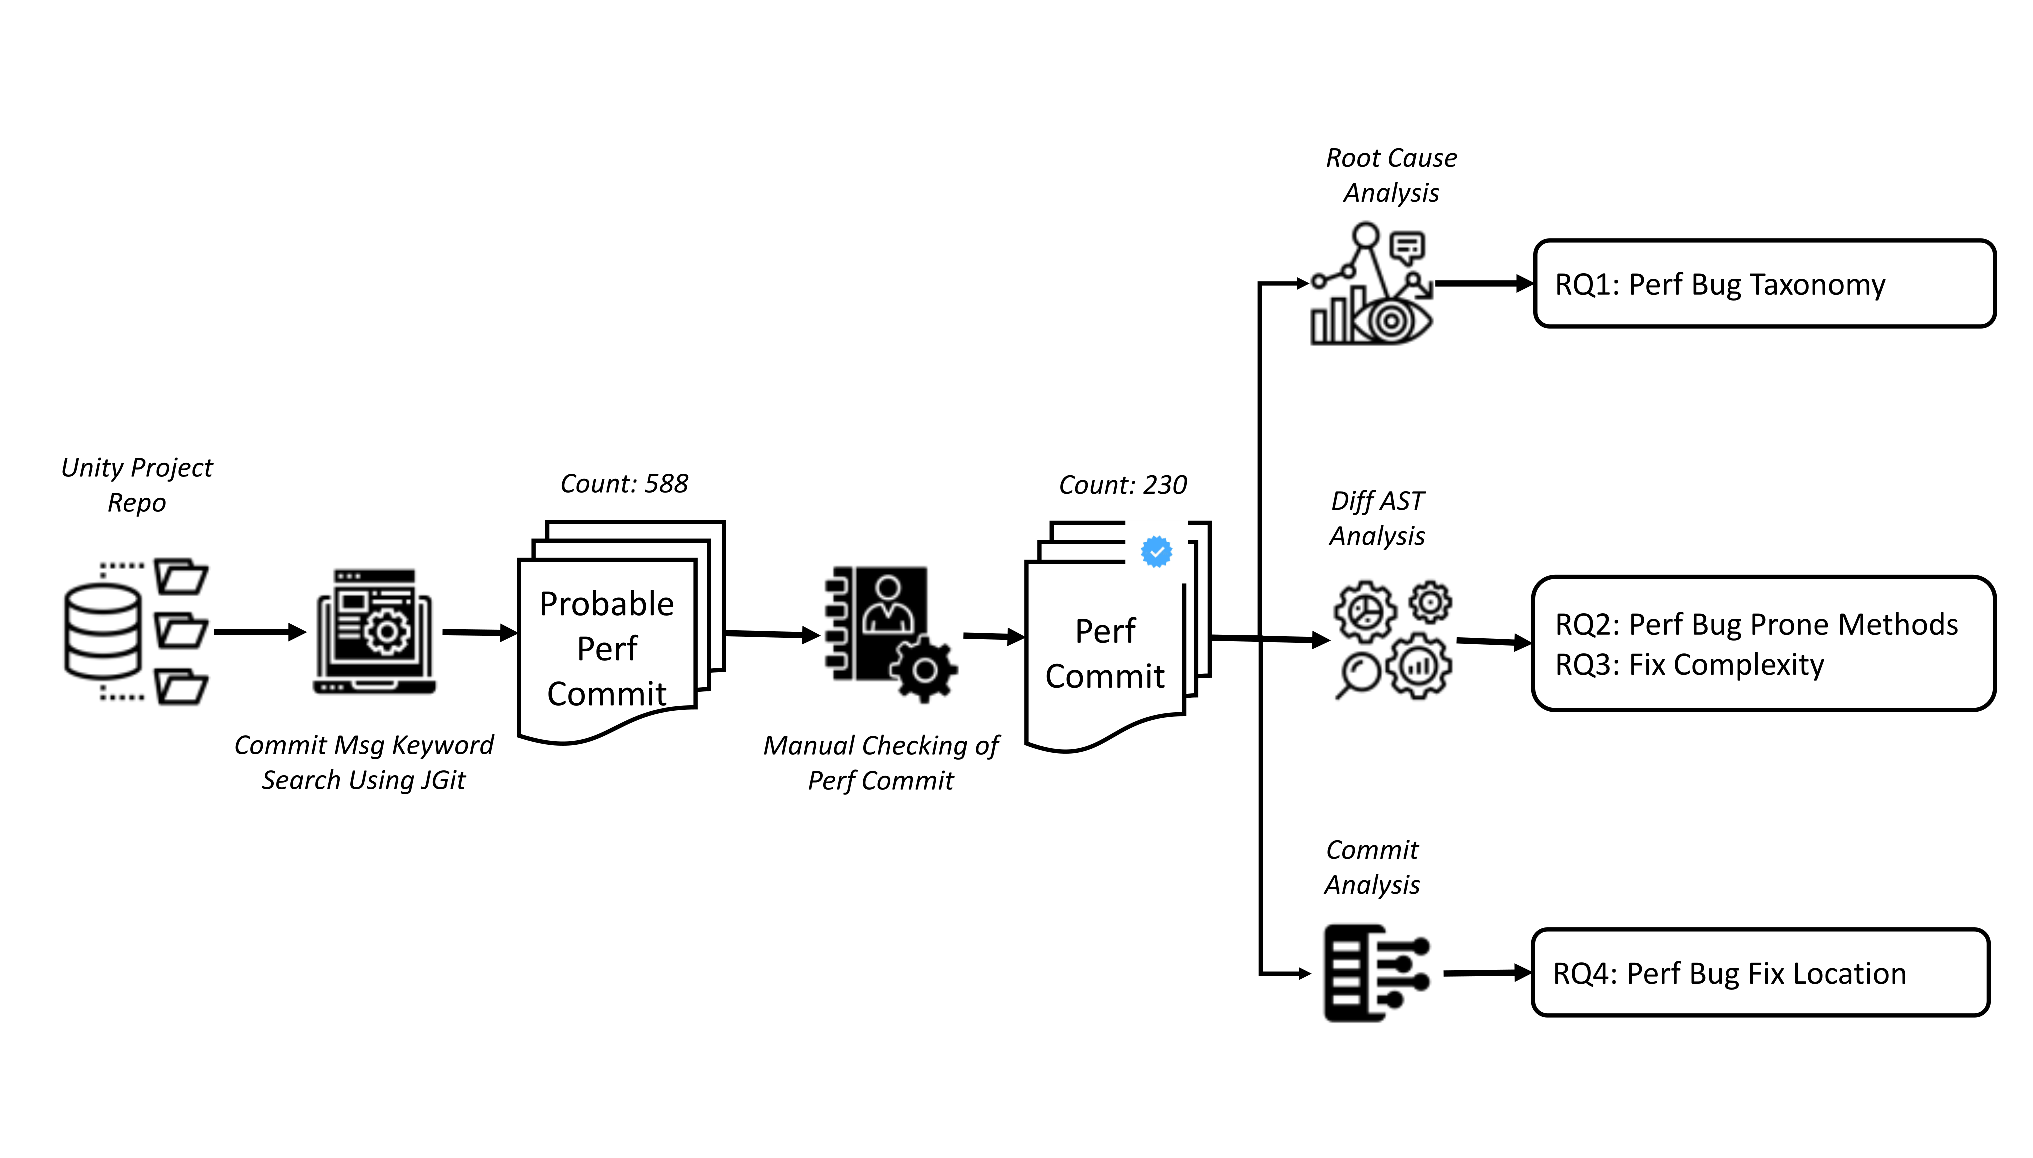
\includegraphics[width=0.9\textwidth]{figure/overview.eps}
	%\vspace{-0.3cm}
	\caption{Overview of Unity Performance Bug Analysis}
	%	\vspace{-0.3cm}	
	\label{figure:overview}
\end{figure*}

\section{Unity Performance Bug Data Collection}
\label{sec:datacollection}
For Data Collection, we collected 100 Github projects with more than 100 commits. We used the commit threshold to ensure that the projects are well maintained and have sufficient fixed data. With these 100 projects, we programmatically searched for performance fix related keywords in commit message using Java Git library JGit~\cite{JGit}. As part of keyword search, we used \textbf{performance}, \textbf{speed up}, \textbf{accelerate}, \textbf{fast}, \textbf{slow}, \textbf{latency}, \textbf{contention}, \textbf{optimize}, and \textbf{efficient} keywords as search token. Prior research~\cite{Chen:perf:19} on performance bug also used these keywords to find performance related bug fix. With this search strategy, we identified 588 probable performance-related issues. Later we manually checked the commits for the performance-related fix. We checked the commit messages thoroughly and also the fix for performance fix correctness. With our analysis, we identified 230 actual performance related bug fix. Since for Unity, we did not have any dataset for performance analysis, this dataset can contribute to further research on unity performance-related bugs.


\section{Root Cause Analysis}
\label{sec:rootcause}
With detailed root cause analysis, we identified Unity's performance bug fix taxonomy. That means, we categorized the bugs depending on their types and how they got fixed. We categorized these 230 bugs into 15 categories.






\section{Code change-based AST diff analysis}
\label{sec:diffanalysis}
For change/diff based analysis, we performed AST (Abstract Syntax Tree) level diff analysis. For C\# AST tree generation, we did not find any opensource parser. So, we  used srcML~\cite{srcML} a generic parsing research tool. With srcML, we converted C\# code into XML format code. Then we loaded those XML format code and performed AST level diff with the state of the art diff tool GumTree~\cite{Jean:gumtree:2014}. With this approach, we can extract AST level code changes. Figure~\ref{figure:astdiff} shows the overview of C\# AST level diff analysis.

\begin{figure*}[t]
	%%\vspace{-0.2cm}
	\centering
	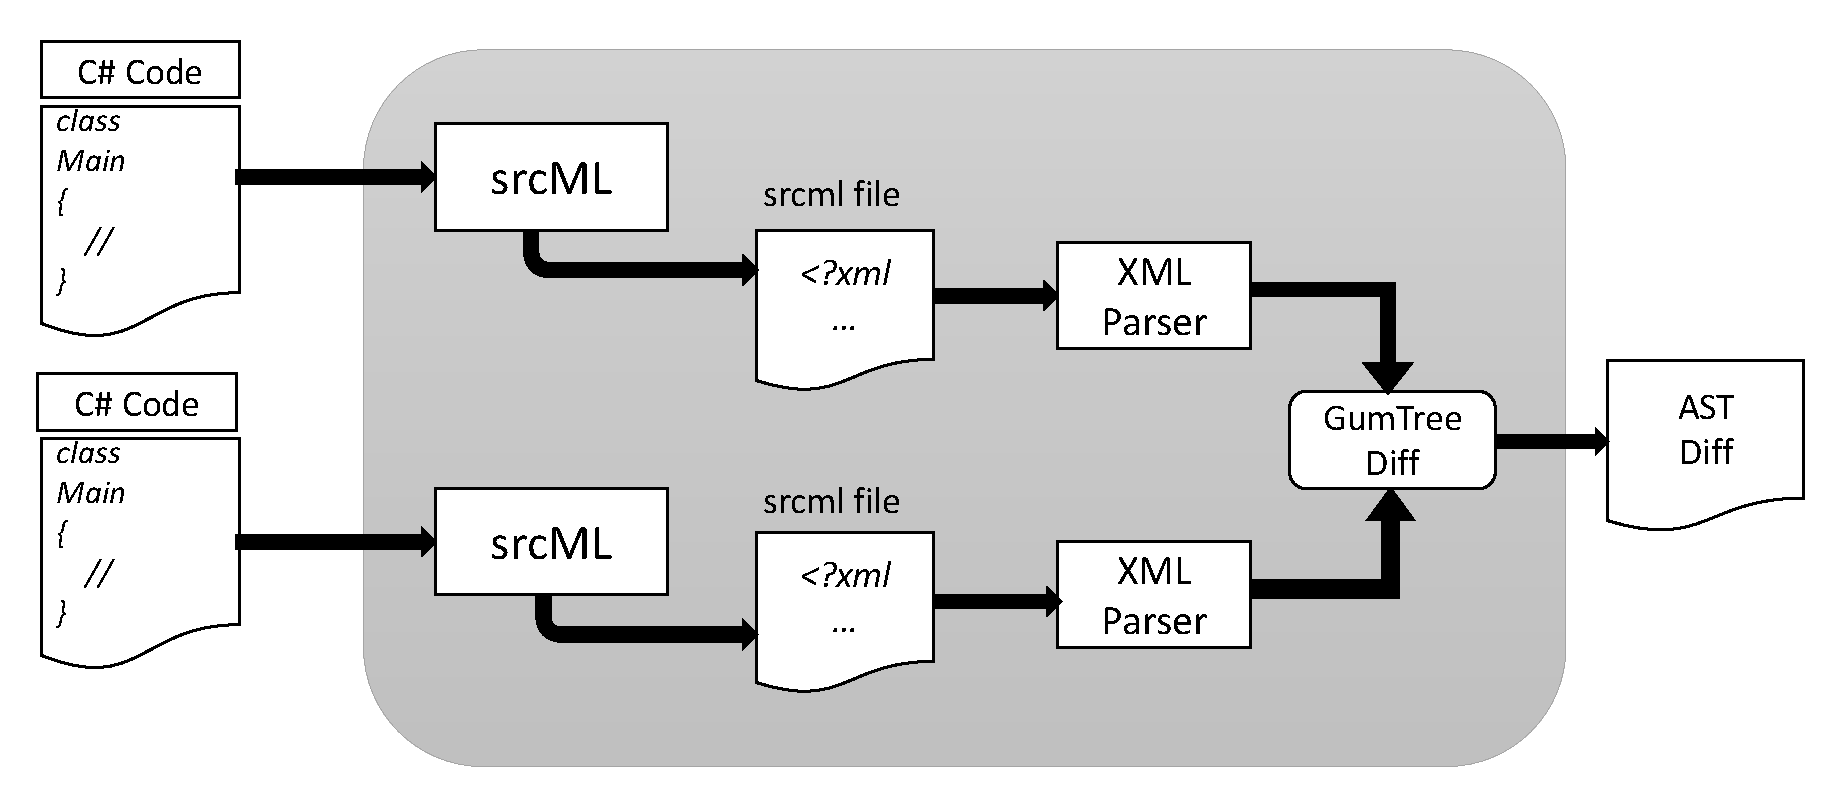
\includegraphics[width=0.9\textwidth]{figure/diff_overview.eps}
	\caption{C\# AST Level Diff Generation}
	\label{figure:astdiff}
\end{figure*}

Here is an example of the AST diff that we generated using our approach. We keep track of class name, method name, action such as insert, delete move etc. Also label and type. For example, here the class name is Answer, no function is used. And there is a single expression, whose type is "using name operator name", and label is "UnityEngine.UI". This "using" in C\# is equivalent to Java "import". Also there is an "insert" action. 


\definecolor{gray}{rgb}{0.4,0.4,0.4}
\definecolor{darkblue}{rgb}{0.0,0.0,0.6}
\definecolor{cyan}{rgb}{0.0,0.6,0.6}

\lstset{
	basicstyle=\ttfamily,
	columns=fullflexible,
	showstringspaces=false,
	commentstyle=\color{gray}\upshape
}

\lstdefinelanguage{XML_android}
{
	morestring=[b]",
	morestring=[s]{>}{<},
	morecomment=[s]{<?}{?>},
	stringstyle=\color{black},
	identifierstyle=\color{darkblue},
	keywordstyle=\color{cyan},
	morekeywords={xmlns,version,type}% list your attributes here
}

\begin{example}
\begin{lstlisting}[language=XML_android, basicstyle=\ttfamily\footnotesize, numbers=left, numbersep=5pt, captionpos=b]
<?xml version="1.0" encoding="UTF-8" standalone="no"?><patch id="3">
	<classname name="Answer">
		<funcname name="">
			<stmt id="1">
				<exp id="0">
					<type>using name operator name </type>
					<label>  UnityEngine . UI </label>
					<action>insert</action>
				</exp>
			</stmt>
		</function>
	</classname>
</patch>
	\end{lstlisting}
	\caption{C\# Code Differencing Output Format}
		%\scriptsize{\textit{(BuildCraft/BuildCraft: 98f7196)}}}
	\label{example:changerep}
	\vspace{-0.2cm}
\end{example}

With AST level code changes, we analyzed which methods are prone to performance bug and the complexity of performance bug fix. We categorized performance bug fix methods as Unity Callback, Custom Callback, and User Defined Method during the analysis of performance bug-prone methods. Unity Callbacks are unity provided callbacks such as Update. Update method is called in every frame if the MonoBehaviour is enabled. MonoBehaviour is the base class from which every Unity script derives. Similarly, Start is another Unity callback. Custom callbacks are event listeners that developers can add from code. User-Defined Methods are other utility or supporting methods that are used in unity scripts. Apart from that, we also performed analysis for most frequently changed methods. During the most common method change analysis, we performed analyses based on only method body changed based analysis and also method body considering call graph-based analysis.



\section{Commit Analysis}
\label{sec:commitanalysis}
In typical bug fix, we do have a normal illusion that performance bugs are mostly fixed in source code. To analyze the factor, we analyzed the performance fix location. So for the 230 performance bugs, we analyzed git commit. We captured the Delta or change in between bug fix commit and its parent commit. From Delta, we identified which files are changed. Based on file type change, we categorized fix location. We did this analysis programmatically with the help of Git Java library JGit. Figure~\ref{figure:commitanalysis} shows the overview of commit analysis.

\begin{figure*}[t]
	%%\vspace{-0.2cm}
	\centering
	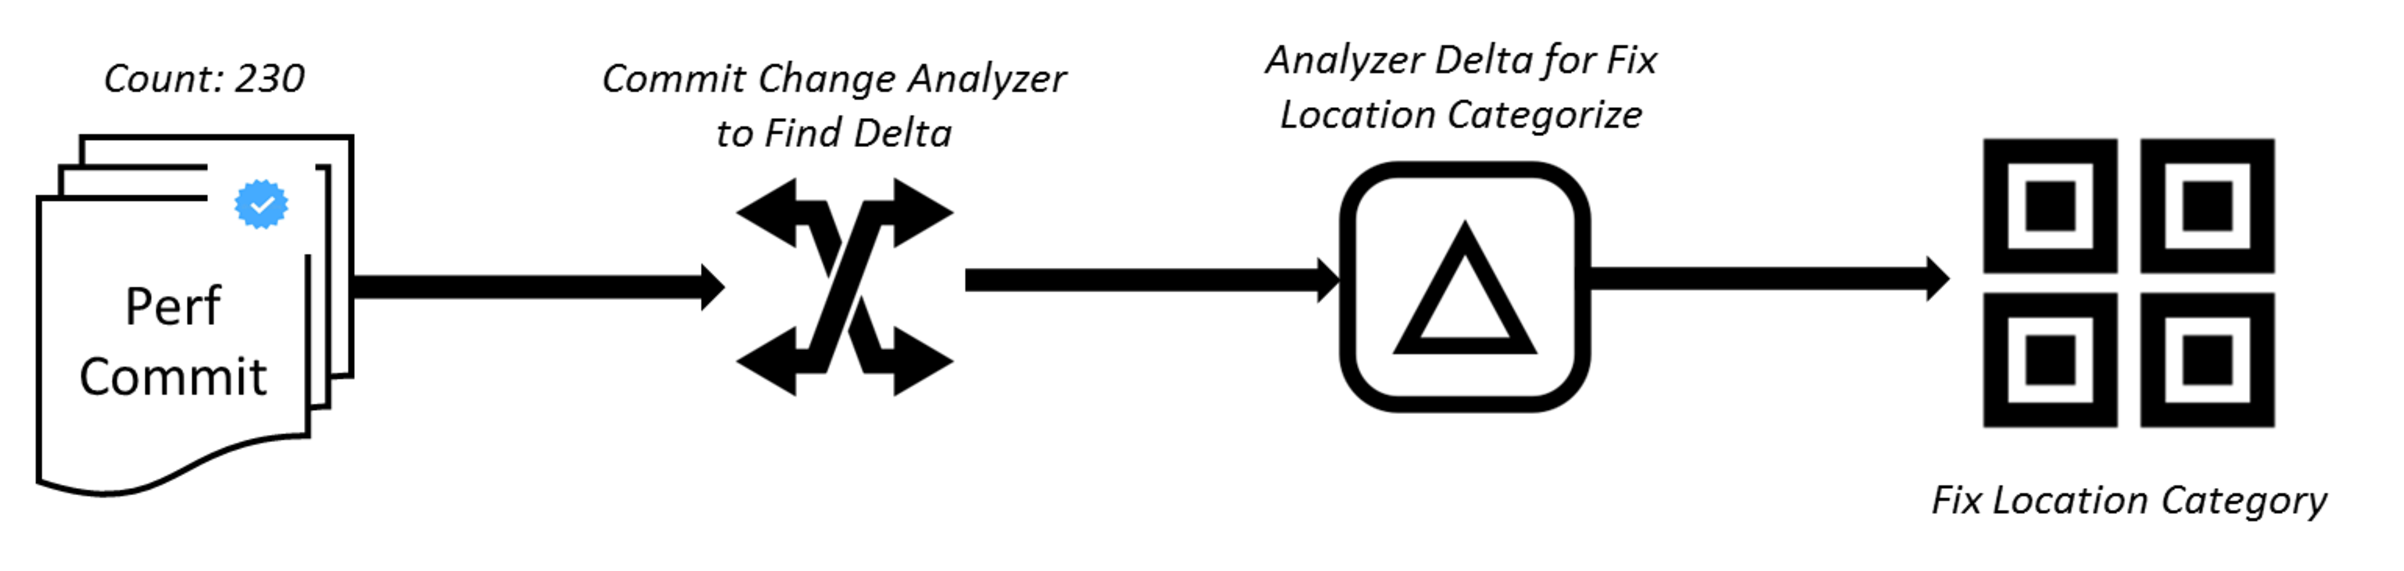
\includegraphics[width=0.9\textwidth]{figure/commitanalysis.eps}
	%\vspace{-0.3cm}
	\caption{Overview of Commit Analysis}
	%	\vspace{-0.3cm}	
	\label{figure:commitanalysis}
\end{figure*}


\chapter{EMPIRICAL EVALUATION}
\label{chapter:empevaluation}
In this section, we describe our settings in Section~\ref{sec:settings}, followed by research questions in Section~\ref{sec:rqs}. Finally, we discuss experiment results in Section~\ref{sec:results}

\section{Experiment Settings}
\label{sec:settings}
We collected a dataset of 100 GitHub projects described in Section~\ref{sec:datacollection}. For performance commit identification and code change analysis, we use a computer with 2.4 GHz Intel Core i7 CPU with 16GB of Memory, and Ubuntu 14.10 LTS operating system. 

\section{Research Questions}
\label{sec:rqs}
In our analysis, we seek to answer following research questions. 

\begin{itemize}
	\item \textbf{RQ1:} What are the major root causes of \unity performance bugs?
	
	\item \textbf{RQ2:} What are the most common performance bug prone methods of \unity performance bugs?
	
	\item \textbf{RQ3:} How difficult is to fix \unity performance bugs?
	
	\item \textbf{RQ4:} Which files are common to resolve \unity performance bugs?
\end{itemize}


\section{Results}
\label{sec:results}

\subsection{RQ1:Root Causes of Unity Performance Bugs}
\label{subsec:rootcause}
With detailed root cause analysis, we identified Unity's performance bug fix taxonomy. That means, we categorized the bugs depending on their types and how they got fixed. We classified these 230 bugs into 15 categories. Figure~\ref{figure:rq1category} shows the Unity performance bug taxonomy with their frequency. Among these 230 performance  bugs, largest category is Asset/Prefab related optimization. In Unity game components are stored in asset file and for reusability some assets are  bundled together and used as prefab file. 18 fixes are related to loop optimization and 16 fixes are related to caching related fix. Data Structure related performance fixes accounts for 16 cases. Other fixes are: Don't use var, avoid linq and regx, string operation, use of readonly and constant, Memory cleanup, move unnecessary code, Run code in every X frame and thread related fixes. Performance fixes that we cannot generalized are considered as Others type. 


\begin{figure*}[t]
	%%\vspace{-0.2cm}
	\centering
	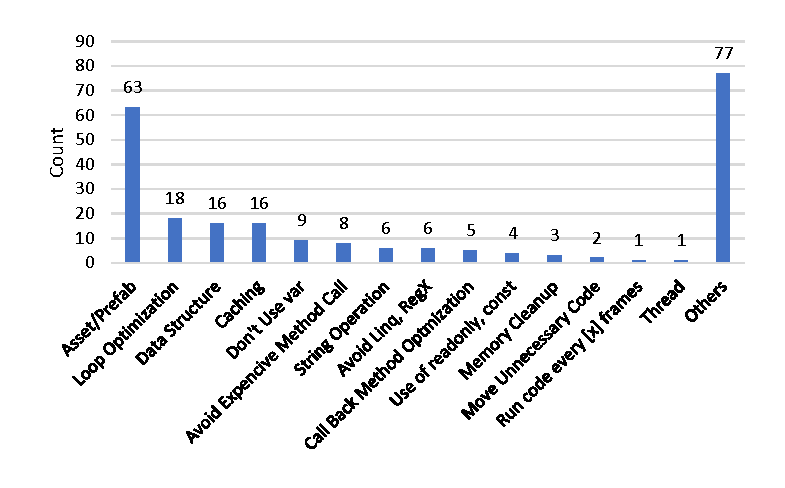
\includegraphics[width=0.8\textwidth]{figure/rq1_taxonomy.eps}
	%\vspace{-0.3cm}
	\caption{Unity Performance Bug Taxonomy with Frequency}
	%	\vspace{-0.3cm}	
	\label{figure:rq1category}
\end{figure*}

In the following subsections, we will discuss detail about each of the bug category.

\subsubsection{Asset/Prefab Bug Fix}
The graphical parts of the game can primarily impact two computer systems: the GPU and the CPU. Considering that, a major portion of Unity Performance bugs are related to Asset or Prefab optimization. Example~\ref{example:taxonomy1} shows such an example of a performance bug fix. In this fix, developers improved performance prefab that is bundling related components as a bundle. We check the unity documentation too that uses of prefab are helpful for performance improvement.

\begin{example}
	\begin{lstlisting}[escapechar=!]	
	!\colorbox{light-green}{+\-\-\- \!u\!1001 \& 1246218760}!  
	!\colorbox{light-green}{+Prefab:}! 
	!\colorbox{light-green}{+         m\_ObjectHideFlags: 0}! 
	!\colorbox{light-green}{+         serializedVersion: 2}! 
	!\colorbox{light-green}{+     		m\_Modification:}! 
	!\colorbox{light-green}{+				m\_TransformParent: {fileID: 713704410}}!      
	\end{lstlisting}
	\caption{Asset/Prefab Related Fix
		\scriptsize{\textit{(AdrianBZG/Medieval\_Warfare\_VR\-Unity:207bc51)}}}
	\label{example:taxonomy1}	
\end{example}
 
\subsubsection{Loop Optimization}
In \unity use of typical "for" loop instead of "foreach" helps to improve performance. We also check several Stackoverflow issues to confirm this fix. So, for Unity it's suggested to use "for" rather than foreach.



\begin{example}
\begin{lstlisting}[escapechar=!]
!\hlp{- foreach (VRTK\_BasicTeleport teleporter in VRTK\_ObjectCache.registeredTeleporters)}!   
!\hlg{+ for (int i = 0; i < VRTK\_ObjectCache.registeredTeleporters.Count; i++)}! 
{
!\hlg{+VRTK\_BasicTeleport teleporter = VRTK\_ObjectCache.registeredTeleporters[i]; }!
teleporter.Teleporting -= new TeleportEventHandler(OnTeleporting);
\end{lstlisting}
  \caption{Loop Optimization
  	\scriptsize{\textit{(gpvigano/VRTK-GearVR-Test:c2c9e08)}}}
  \label{example:diff}  
\end{example}


\subsubsection{Caching-Based Performance Fix}
Caching is the process of storing data in memory or data structure. In Example~\ref{example:caching}, rather than loading gameobject again and again. Dictionary is used to save a copy of the already loaded gameobject. This works as a singleton pattern if not created, then create otherwise return existing instance. Caching is widely used in performance optimization of Unity applications. 

\begin{example}
\begin{lstlisting}[escapechar=!]
!\hlg{+private static Dictionary<string, GameObject> objects = new Dictionary<string, GameObject>();}!
...
!\hlg{+    GameObject FastResource(string resource) \{ }!
!\hlg{+        if (\!objects.ContainsKey(resource)) \{}!
!\hlg{+            objects.Add(resource, (GameObject) Resources.Load(resource));}!
!\hlg{+        \}}!
!\hlg{+        return objects[resource];}!
!\hlg{+ \}}!
...
GameObject CreateFace(Vector3 localPosition, Vector3 scale, Vector3 angles, string type){
...
!\hlp{-        var frontSide = (GameObject)GameObject.Instantiate(Resources.Load(type));}!
!\hlg{+        var frontSide = (GameObject)GameObject.Instantiate(FastResource(type));}!
}
\end{lstlisting}
  \caption{Caching-based Performance Fix
  	\scriptsize{\textit{(stefaanvermassen/virtual-museum-app:b3823da)}}}
  \label{example:caching}  
\end{example}


\subsubsection{Data Structure Related Fix}
The data structure is a particular way of storing data in a computer. Developers must choose the appropriate data structure for better performance. Example~\ref{example:dt} shows a performance fix using right Data Structure. Since this data structure code is always using the first element, so, rather than using a list, the LinkedList is much more effective to get the first item. We got similar issues like using Maps where required.


\begin{example}
\begin{lstlisting}[escapechar=!]
!\hlp{-     private List<GazeSample> stabilitySamples = new List<GazeSample>();}!
!\hlg{+     private LinkedList<GazeSample> stabilitySamples = new LinkedList<GazeSample>();}!
...

!\hlp{- if (stabilitySamples.Count >= StoredStabilitySamples)}!
!\hlg{+                // Remove from front items if we exceed stored samples.}!
!\hlg{+                while (stabilitySamples.Count >= StoredStabilitySamples)}!
					   {
!\hlp{-                    stabilitySamples.RemoveAt(0);}!
!\hlg{+                    stabilitySamples.RemoveFirst();}!
          				}
\end{lstlisting}
  \caption{Data Structure Related Performance Fix
  	\scriptsize{\textit{(stefaanvermassen/virtual-museum-app:b3823da)}}}
  \label{example:dt}  
\end{example}


\subsubsection{Don't Use Var}
It indicates that it is better to use concrete data type rather than using generic data type var. If the compiler cannot determine exact type of type data pointing to var, then it might create compilation error. Apart from that run time type determination might have performance overhead.


\subsubsection{Avoid expensive method call}
There are some methods that are considered as expensive by the developers, such as GetComponent. In Unity, it is common is to call GetComponent to access components. In many cases, developers call GetComponent method inside Update callback to extract components and pass it other methods as parameter. To improve the performance, we can extract all the components in Start callback and reuse the components. This will reduce the repitative GetComponent method call.

\subsubsection{Avoid Linq, Regx}
LINQ is a structured query syntax built in C\# to retrieve data from different types of data sources. Regx represents regular expressions. It is suggested to avoid Linq and regx.  

\subsubsection{String Operation}
For string concatenation, string boxing, we had to use string builder rather than string append function. In C\#, Strings are immutable, which means that after creation if the value is changed it allocate new memory space. Repetitive String value update, concatenation creates lot of garbage. To improve the performance, we should cut down on unnecessary string creation and manipulation. If String value is determined during runtime, it's better to use StringBuilder class. Similarly, we should avoid boxing such as String.Format() method that takes a String and an object parameter. Boxing creates garbage because of what happens behind the scenes. When a value-typed variable is boxed, Unity creates a temporary System.Object on the heap to wrap the value-typed variable. Boxing might create unnecessary memory overhead.


\subsubsection{Callback method optimization}
We should remove any expensive calculation and unnecessary things from callback methods. Also, we should remove any empty callback method. Update(), LateUpdate(), and other event functions look like simple functions, but they have a hidden overhead. They do have hidden overhead communication between Unity engine code and managed code. Apart from that, Unity performs additional safety checking before initiating these methods. For a single method, the overhead might not be noticeable, but accumulatively it can create performance overhead.


\subsubsection{Use of readonly, constant}
4 fix indicates that using readonly, constant improves performance. The use of readonly generates immutable data structures. Immutable data structures cannot be changed once constructed. This makes it very easy to reason about the behavior of a structure at runtime. A const can be optimized by the compiler to be inlined into the code.

\subsubsection{Memory cleanup}
This is something about cleaning up the game object/ data structure in the destructor. When the variable goes out of scope, garbage collector identifies and deallocates unused heap memory. The garbage runs behind the process to clean up memory periodically. But for the case where Unity developers allocated large block of memory, it might take time to deallocate the memory by the garbage collector. So, to improve the performance, it's better to deallocate memory in the intended time.

\subsubsection{Move Unnecessary Code}
Writing efficient code and structuring it wisely can lead to improvements in Unity application performance. Loops can be one area where developers can rule out unnecessary code from the loop. In that line choosing wise loop condition and if a code is not required execute in a loop we should move the code outside the loop. Also, by using "if-else" we can stop the execution of some unnecessary code. 



\subsubsection{Run code every [x] frame}
If a code block needs to execute frequently and triggered by an event, it may not be necessary to run every frame. In Example~\ref{example:runcode1}, ExampleExpensiveFunction method is called in every frame and it might be costly to execute the program. In case if the method is not mandatory to execute in every frame, then it might be helpful by executing in some interval. Example~\ref{example:runcode2} shows such an optimized version of code where ExampleExpensiveFunction method is called in every 3 frames.

\begin{example}
\begin{lstlisting}[escapechar=!]
void Update()
{
    ExampleExpensiveFunction();
}          				}
\end{lstlisting}
  \caption{Run Code Everytime Example}
  \label{example:runcode1}  
\end{example}

\begin{example}
\begin{lstlisting}[escapechar=!]
private int interval = 3;

void Update()
{
    if (Time.frameCount % interval == 0)
    {
        ExampleExpensiveFunction();
    }
}
\end{lstlisting}
  \caption{Run Code Every [3] Frame Example}
  \label{example:runcode2}  
\end{example}


\subsubsection{Thread}
In multi-threading program two of multiple parts can run concurrently and each code block can handle a different task at a time. In threading based optimization programs can load game components in multiple threading or render in multiple threads. In some cases optimization can be  done through making any thread asynchronous from synchronous to reduce thread waiting time. 
 

\subsection{RQ2:Bug Prone Methods}
\label{subsec:bugmethod}
Based on our code change diff analysis discussed in Section~\ref{sec:diffanalysis}, we identified which methods are changed. We categorized these methods as Unity Callback, Custom Callback, and User Defined Method. Unity Callbacks are unity provided callbacks such as Update. Update is called in every frame if the MonoBehaviour is enabled. MonoBehaviour is the base class from which every Unity script derives. Similarly, Start is another Unity callback. Custom callbacks are event listeners that developers can add from code. User-Defined Methods are other utility or supporting methods that are used in unity scripts. Figure~\ref{figure:rq2methodtype}shows the frequency of each type of method in our diff based change analysis. Based on our analysis, Unity callback is changed 224 times, while custom callbacks are changed 409 times. In the case of user-defined methods, those are changed 2706 times.

\begin{figure*}[t]
	%%\vspace{-0.2cm}
	\centering
	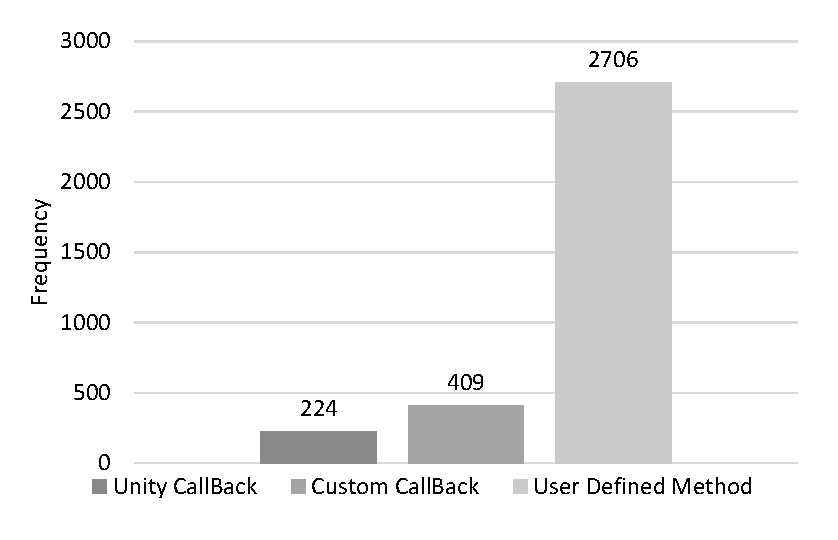
\includegraphics[width=0.8\textwidth]{figure/rq2_1.eps}
	%\vspace{-0.3cm}
	\caption{Type of Methods Prone to Performance Bug}
	%	\vspace{-0.3cm}	
	\label{figure:rq2methodtype}
\end{figure*}

Apart from that, we identified the top 10 frequently changed methods. If any method body is altered, we considered that the method is changed. As shown in the Figure~\ref{figure:rq2fixmethod}, Update method changes most frequently. Others are Start, Awake, OnEnable, etc. From the analysis, we identified that unity callbacks are related to performance bug locations. So, these methods are updated frequently. In this analysis, we did not consider callgraph dependency.

\begin{figure*}[t]
	%%\vspace{-0.2cm}
	\centering
	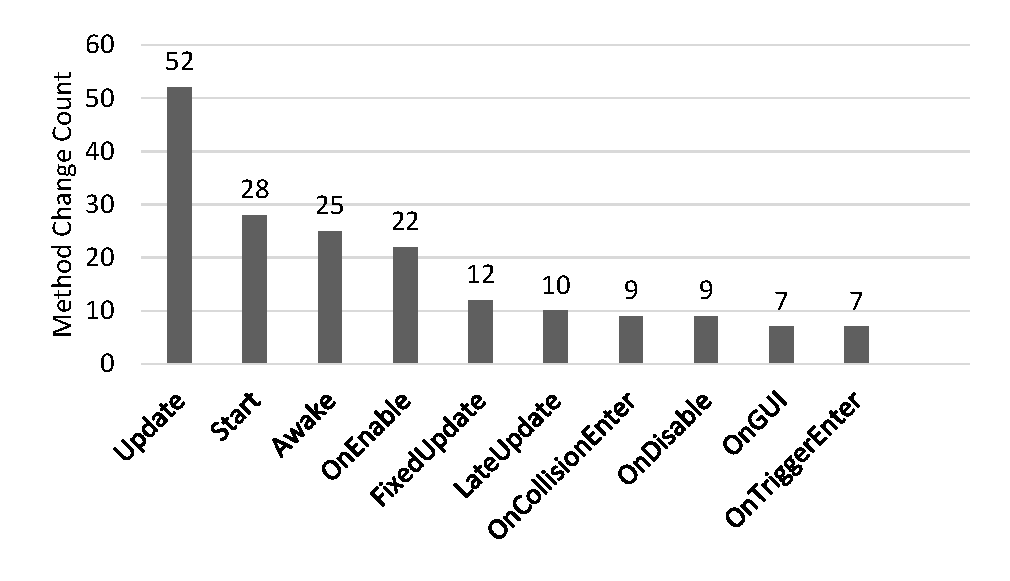
\includegraphics[width=0.8\textwidth]{figure/rq2_2.eps}
	%\vspace{-0.3cm}
	\caption{Fix Methods Without Considering Call Graph}
	%	\vspace{-0.3cm}	
	\label{figure:rq2fixmethod}
\end{figure*}


Later we did another analysis considering the code change method and static call graph dependency. According to the call graph figure, if a method is changed, then dependent methods are also considered as changed due to caller callee relationship. When we consider call graph dependency, we identified that the frequency of Unity callbacks also increased. That indicates that user-defined methods that are called from Unity callbacks are prone to performance bugs. Figure~\ref{figure:rq2fixmethodcallgraph} shows the frequency of Method change frequency based on code change and call graph dependency. 

\begin{figure*}[t]
	%%\vspace{-0.2cm}
	\centering
	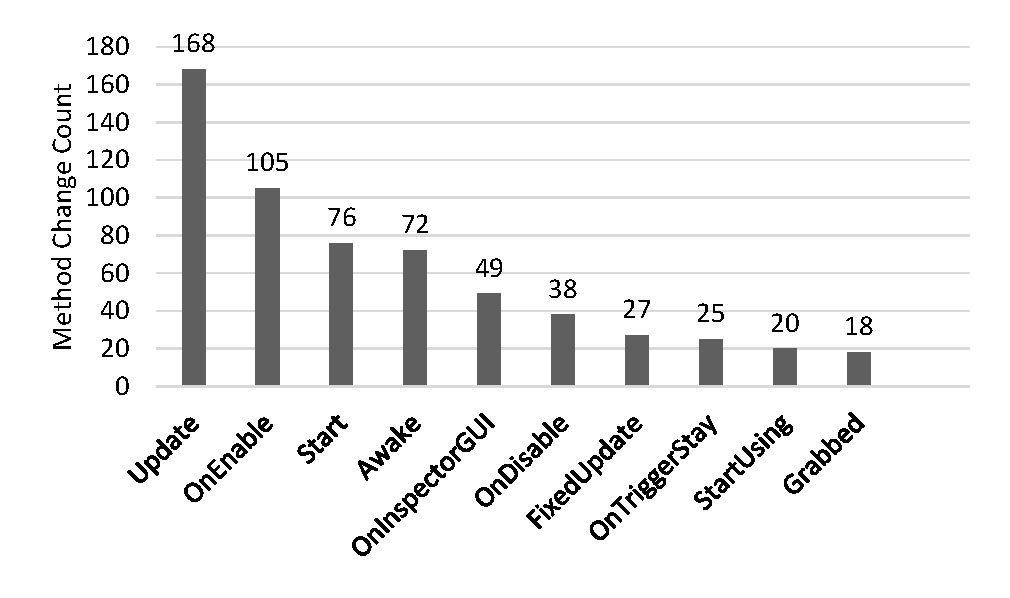
\includegraphics[width=0.8\textwidth]{figure/rq2_3.eps}
	%\vspace{-0.3cm}
	\caption{Fix Methods Considering Call Graph}
	%	\vspace{-0.3cm}	
	\label{figure:rq2fixmethodcallgraph}
\end{figure*}

If we consider distinct method changes contributed to 230 performance bugs, for 77 bugs, there is a change in the Update method; for 41 bugs, Start method is changed. OnInspectionGUI method changed in 39 bugs. Like other analyses, we also found the majority of the bugs fixes are related to callback methods. Figure~\ref{figure:rq2distinctmethod} shows the top 10 methods that contributed to performance bug fix.


\begin{figure*}[t]
	%%\vspace{-0.2cm}
	\centering
	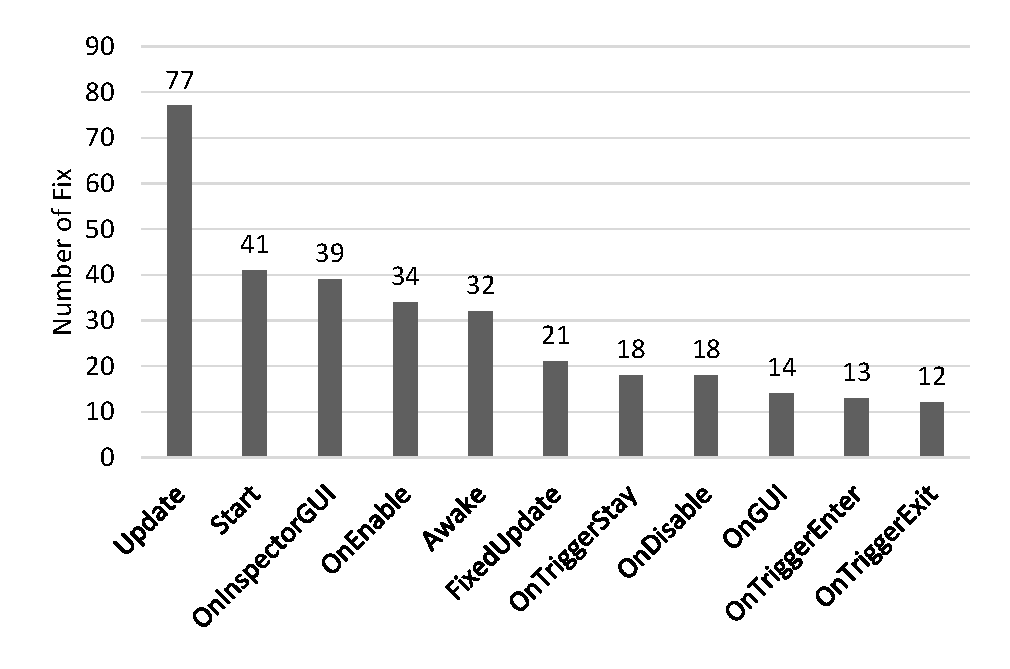
\includegraphics[width=0.8\textwidth]{figure/rq2_4.eps}
	%\vspace{-0.3cm}
	\caption{Individual Method Contribution to Fix Performance Bugs}
	%	\vspace{-0.3cm}	
	\label{figure:rq2distinctmethod}
\end{figure*}


\subsection{RQ3:Performance Fix Complexity}
\label{subsec:bugcomplexity}

Based on code change, we measured the Performance Fix Complexity. In terms of class change, the average class change per performance bug is 3.73, and the median is 1.00. For the case of MethodChange, the size average method change is 12.80 method, and the median is 3.50.  For statement change average statement change count is 32.83, and the median is 10.50. Figure~\ref{figure:rq2distinctmethod} shows the performance fix complexity distribution. From this analysis, we can confer that performance fixes are complex in nature.

\begin{figure*}[t]
	%%\vspace{-0.2cm}
	\centering
	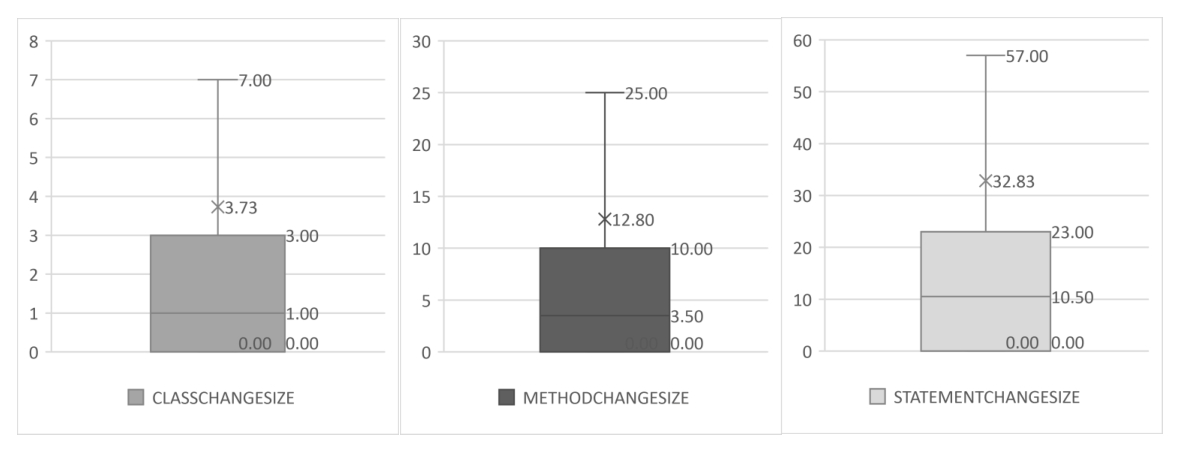
\includegraphics[width=0.9\textwidth]{figure/rq3_1.eps}
	%\vspace{-0.3cm}
	\caption{Performance Fix Complexity Distribution}
	%	\vspace{-0.3cm}	
	\label{figure:rq3}
\end{figure*}

Here some of the reasons why performance fixes are complex in nature. The most common reason is code and component dependency. So, if we change in one method or class, then in most cases, it's required to change in code dependency.  Another reason we observed that in many cases, developers fix several performance issues altogether.  For example, we found that when performing loop optimization, developers optimize loop related fixes in several locations. Two other reasons are lack of tool support and documentation. So, performance issues cannot be identified early. Later based on block or StackOverflow, developer refactors code. Since issues are identified later, code refactoring size becomes large.

\subsection{RQ4:Performance Bug Fix Location}
\label{subsec:bugcomplexity}
Based on the analysis of change(see Section~\ref{sec:commitanalysis}), here is the categorized result of performance bug fix location. As shown in Figure~\ref{figure:rq4}, 92 bugs are fixed by changing only in source code. Forty-five bugs require a change in unity asset or prefab file change. But 93 bugs required to change in both source and unity asset/prefab files. This is critical findings that, to improve or fix performance in many cases, we need to change asset/prefab files. So, the performance analysis of asset/prefab is also important.

\begin{figure*}[t]
	%%\vspace{-0.2cm}
	\centering
	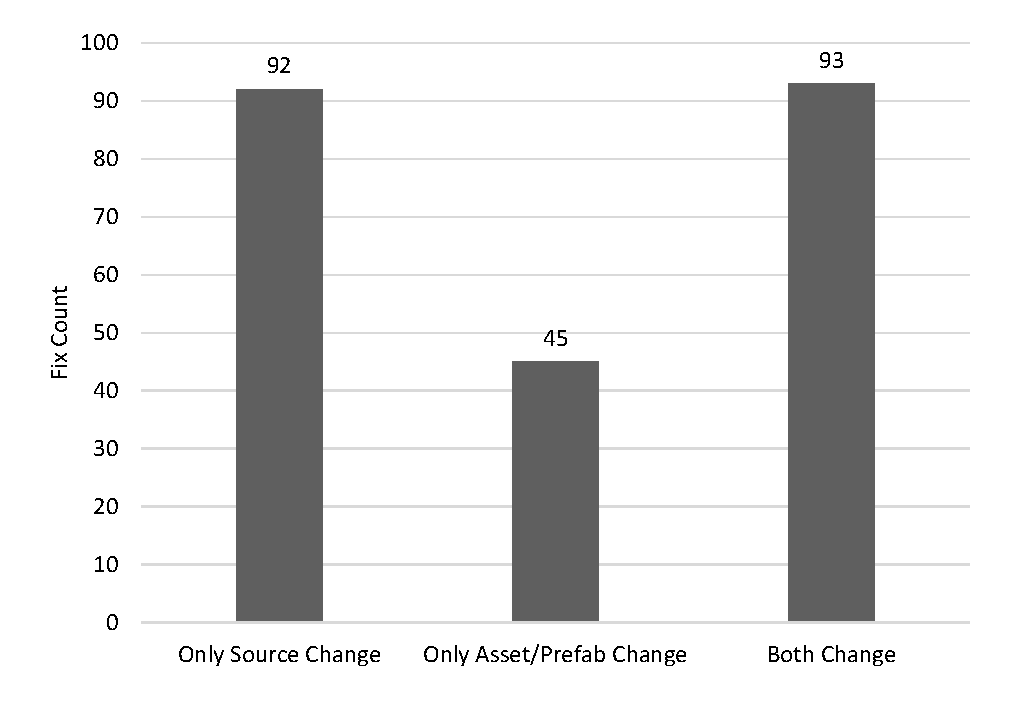
\includegraphics[width=0.9\textwidth]{figure/rq4_1.eps}
	%\vspace{-0.3cm}
	\caption{Performance Bug Location}
	%	\vspace{-0.3cm}	
	\label{figure:rq4}
\end{figure*}


\begin{example}
\begin{lstlisting}[escapechar=!]
!\hlp{-o.pos = mul(UNITY\_MATRIX\_MVP, v.vertex);}!
!\hlg{+o.pos = UnityObjectToClipPos(v.vertex);}!
\end{lstlisting}
  \caption{Example of Asset/Prefab Related Fix
  	\scriptsize{\textit{(RussellXie7/Unity\_Hololens\_Dev:b3823da)}}}
  \label{example:asset1}  
\end{example}

Example~\ref{example:asset1} shows such a performance fix where UnityObjectToClipPos routine is used to calculate Transformation of plane. Unity documentation also mentioned that mul routine could also be used for the Transform plane, but UnityObjectToClipPos is a more efficient way to calculate the plane.

\chapter{Discussions}
\label{chap:discussions}
\section{Threats of Validity}
\label{sec:threats}
The major threat to the internal validity of our analysis is the correctness of manual categorization of performance bug types. To reduce this threat, we carefully performed all these processes and cross-checked fix types in StackOverflow and Unity documentation for the correctness. The major threat to the external validity of our analysis is that our findings may be project-specific of our analysis dataset. To reduce this threat, we used projects with sufficient commit history and are well maintained.


\section{Take Away from the Analysis}
\label{sec:takeway}
Unity performance bug taxonomy shows different bug categories that can be useful for bug detection and repair suggestions. Our analysis also identifies several programming language features such as using readonly, const that can be helpful for performance improvement. AST-based diff analysis identifies that Unity callback methods are prone to performance bugs. So, developers should give extra attention while adding code to the callback methods. Code change empirical data also indicates that Unity performance bugs are complex in nature and require to change in multiple code locations. Finally, commit analysis identifies that performance bugs can happen due to Unity GameObject Asset/Prefab Issues. 





\chapter{Related Work}
\label{chap:relatedwork}

\section{Empirical Studies of Performance Bugs}
\label{sec:empperformance}
Since performance is one of the critical non-functional requirements of software systems, a number of studies analyzed the performance bug of software systems. Zaman et al.~\cite{zaman_security_2011} did a bug analysis of generic bugs collected from Firefox web browser. Their study focused on security and performance bugs of Firefox web browser. Their followup work~\cite{Zaman_study_2012} analyzed the bug reports of Firefox and Chrome to differentiate characteristics performance and non-performance bugs. To identify performance bug code patterns, Jin et al.~\cite{Jin_performance_2012} did root cause analysis of 109 performance bug collected from five projects. Nistor et al.~\cite{Nistor_performance_2013} did a study on performance and non-performance bugs from three popular codebases: Eclipse JDT, Eclipse SWT, and Mozilla. Recent study~\cite{Chen:perf:19} on 700 performance bug fixing commits across 13 popular open-source projects characterizes the relative frequency of performance bug types as well as their complexity. Prior works on performance bugs focused on generic performance bug categorization. But in our study, we tried to focus on Unity performance bug taxonomy and complexity that can be helpful for developers and further research on identifying performance bugs.


\section{Empirical Studies of Generic Bugs}
\label{sec:genericbug}
There are several research works~\cite{Fonseca2010, Lu2008, Sahoo2010} that study and characterize different aspects of generic bugs. Park et al.~\cite{Park2012} did a study focusing on bugs that need more than one fix attempt. Asaduzzaman et al. ~\cite{Asaduzzaman2012} mined the bug introducing changes in the Android platform to identify problematic changes. Aranda et al. ~cite{Aranda2009} did a study on common bug fixing coordination patterns and to provide implications for software engineering tool developers.


\section{Performance Bug Detection}
\label{sec:detection}
Since performance issues are difficult to detect, several research works focused on identifying performance bugs. Several techniques~\cite{Siegmund2012, Killian2010, Yan2012} adopted to detect performance bugs. Recent work~\cite{Mostafa2017} focused on regression performance test case selection to detect bugs early. Han et al.~\cite{Han2018} utilize Machine Learning to generate test frames for guiding actual performance test case generation. While Chen et al.~\cite{Chen2014} discussed performance Anti-Patterns for applications.




\chapter{CONCLUSION AND FUTUREWORK}
\label{chap:conclusion}
In this study, we did an empirical analysis on \unity performance bugs derived from 230 performance bug fixing commits across 100 open source projects written in Unity. We manually investigated these commits to confirm that the fixes are related to Unity performance bugs.  In summary, we generated Unity performance bug taxonomy and Unity callback methods prone to performance bugs. Apart from that, our analysis performance bugs fix complexity identifies that \unity performance bugs are complex in nature and require to change in multiple code locations. Our commit change analysis also figured out that performance bugs can happen due to Unity GameObject Asset/Prefab Issues. As far as our knowledge, this is the first work on Unity performance bugs  and this work will be helpful for developers and researchers to identify performance issues.

In the future, we plan to generate a taxonomy of Unity asset or prefab related performance issues. Based on our current findings of code related performance bugs and asset-related finding, we plan to develop an analyzer to detect performance-related bugs. We also planned to build a tool to provide performance bug fix suggestions. 




%\chapter{Ontologies}
%\renewcommand{\bibname}{Appendix}
\begin{center}
\section*{Appendix}
\end{center}
Dataset and Source Code: \url{https://github.com/Fariha1502/unityperfanalyzer}

\pagebreak{}
\renewcommand{\bibname}{BIBLIOGRAPHY}

\bibliographystyle{plain}
\nocite{*}
\bibliography{sampleThesis}

\begin{vita}
Fariha was born and brought up in Bangladesh, a small, beautiful country in South Asia. She earned her bachelor degree in Computer Science and Engineering from the Military Institute of Science and Technology(MIST), Bangladesh. She enrolled in the Master's program at The University of Texas at San Antonio (UTSA) in Fall 2017. As part of the Master's thesis, she started working under the supervision of Dr. Xiaoyin Wang. Her main research interest is in the performance optimization of AR and VR applications. She has been awarded UTSA Computer Science award, a competitive scholarship for her outstanding results. 
%There can be more paragraphs.
\end{vita}

\end{document}
